\documentclass[aspectratio=1610,12pt]{beamer} %Other possible values are: 169, 149, 54, 43 and 32.

% Preambulo com pacotes para o documento

% Pacotes de Matemática
\usepackage{amsmath}    % Melhora a formatação de fórmulas matemáticas
\usepackage{amsthm}     % Facilita a criação e formatação de teoremas
\usepackage{amsfonts}   % Fontes matemáticas adicionais
\usepackage{amssymb}    % Símbolos matemáticos adicionais
\usepackage{amscd}      % Diagramas de comutatividade
\usepackage{mathrsfs}   % Fonte cursiva para símbolos matemáticos
\usepackage{bbm}        % Fonte Blackboard Bold

% Pacotes de Algoritmos e Programação
\usepackage[ruled,lined]{algorithm2e}   % Para criar algoritmos e pseudocódigos

% Pacotes para Texto e Layout
\usepackage{caption}    % Personaliza legendas de figuras e tabelas
\usepackage{microtype}  % Melhora a tipografia
\usepackage{todonotes} % Adiciona notas e lembretes
\usepackage{lipsum}     % Gera texto de exemplo (Lorem Ipsum)
\usepackage{geometry}   % Configura margens e dimensões de página
\usepackage{ragged2e}   % Ajusta a justificação do texto
\usepackage{multicol}   % Divide o texto em várias colunas
\usepackage{pdfsync}    % Sincroniza PDF com código-fonte
% \usepackage{lmodern}    % Usa fontes Latin Modern

% Pacotes para Gráficos e Tabelas
\usepackage{graphicx}   % Inclui e manipula gráficos e imagens
\usepackage{float}      % Melhora o posicionamento de figuras e tabelas
\usepackage{subfig}     % Cria figuras compostas por subfiguras
\usepackage{tabularx}   % Tabelas com largura ajustável
\usepackage{booktabs}   % Melhora a aparência das tabelas com linhas horizontais

% Pacotes para Cores e Estilo
\usepackage{xcolor}    % Extensão do pacote color com mais opções
\usepackage{colortbl}  % Colorir tabelas

% Pacotes para Referências e Bibliografia
\usepackage{biblatex}  % Gerencia bibliografias e citações

% Pacotes para Listas e Enumerações
% \usepackage{enumitem}  % Controle sobre listas enumeradas e com marcadores

% --- Pacote para ÍCONES ---
\usepackage{fontawesome5}

% Outros Pacotes
\usepackage{siunitx}   % Formata unidades e números no Sistema Internacional de Unidades (SI)
\usepackage{url}       % Melhora a formatação e quebra de URLs longos
\usepackage{xspace}    % Gerencia o espaço após macros de texto

\synctex=1 % Habilita SyncTeX

%  Define as cores a serem usadas
\definecolor{UFGblue}{rgb}{0.0039, 0.3529, 0.6431}
\definecolor{UFGred}{HTML}{990000}
\definecolor{UFGorange}{rgb}{0.9216, 0.4863, 0.0784}
\definecolor{UFGgreen}{rgb}{0.0509, 0.4509, 0.1568}
\definecolor{UFGgray}{rgb}{0.3686, 0.5255, 0.6235} % UBC Gray (secondary)
\definecolor{ultramarine}{rgb}{0, 0.125, 0.376}
\definecolor{UFGorange}{rgb}{0.9216, 0.4863, 0.0784}%{HTML}{EB811B}
\definecolor{UFGred}{HTML}{990000}

\definecolor{mybcolor}{rgb}{0.122, 0.435, 0.698}
\definecolor{mygcolor}{rgb}{0.0, 0.7, 0.2}
\definecolor{myrcolor}{rgb}{0.8, 0.0, 0.2}

\definecolor{darkgreen}{rgb}{0.0509, 0.4509, 0.1568}
\definecolor{orangeb}{rgb}{0.9216, 0.4863, 0.0784}%{HTML}{EB811B}
\definecolor{blued}{rgb}{0.0039, 0.3529, 0.6431}

% Comandos para colorir o texto
\newcommand{\red}[1]{\textcolor{UFGred}{#1}}
\newcommand{\blue}[1]{\textcolor{UFGblue}{#1}}
\newcommand{\green}[1]{\textcolor{UFGgreen}{#1}}
\newcommand{\gray}[1]{\textcolor{UFGgray}{#1}}
\renewcommand{\leq}{\leqslant}
\renewcommand{\geq}{\geqslant}

% Criando novos comandos
\DeclareMathOperator{\arsinh}{arsinh}
\DeclareMathOperator{\corr}{Corr}
\DeclareMathOperator{\cov}{Cov}
\DeclareMathOperator{\var}{Var}

% definindo as margens do documento
\geometry{a4paper,text={16.5cm,25.2cm},centering}

% Definindo os conjuntos numéricos 
\newcommand{\C}{\mathbb{C}}
\newcommand{\N}{\mathbb{N}}
\newcommand{\Q}{\mathbb{Q}}
\newcommand{\R}{\mathbb{R}}
\newcommand{\Z}{\mathbb{Z}}


          % Inclui o preâmbulo geral
% 
% Habilita a língua portuguesa
\usepackage[utf8]{inputenc}  % Codificação de entrada para UTF-8
\usepackage[T1]{fontenc}        % Suporte para caracteres acentuados
\usepackage[brazilian]{babel}   % Adapta o documento para o português do Brasil

% Define novos comandos
\DeclareMathOperator{\sen}{sen}
\DeclareMathOperator{\arcsen}{arcsen}
\DeclareMathOperator{\senh}{senh}
\DeclareMathOperator{\arsenh}{arsenh}


% Redefine os comandos para português
\renewcommand{\sin}{\operatorname{sen}\,}
\renewcommand{\sinh}{\operatorname{senh}\,}
\renewcommand{\arcsin}{\operatorname{arcsen}\,}

% Renomeando teoremas para portugues
\theoremstyle{plain}
\newtheorem{teorema}{Teorema}[section]
\newtheorem{axioma}[teorema]{Axioma}
\newtheorem{proposicao}[teorema]{Proposição}
\newtheorem{lema}[teorema]{Lema}
\newtheorem{corolario}[teorema]{Corolário}

% Renomeando definiçoes e exemplos
\theoremstyle{definition}
\newtheorem{definicao}[teorema]{Definição}
\newtheorem{exemplo}[teorema]{Exemplo}
\newtheorem{exercicio}[teorema]{Exerc\'{\i}cio}
% \newtheorem{question}{Questão}

% Renomeando Observações
\theoremstyle{remark}
\newtheorem{observacao}[teorema]{Observação}
\newtheorem{observacoes}[teorema]{Observações}
\newtheorem{notacao}[teorema]{Notação}

% Renomeando Provas e Soluções
\newenvironment{prova}{\vspace{.1cm}\noindent {\red{\bf Prova.}}}{
  $\cqd$\vspace{2mm}}

\newenvironment{solucao}{\vspace{.1cm}\noindent {\green{\bf Solução.}}\footnotesize}{
  $\cqd$\vspace{2mm}}

% Usa o sistema internacional de memidas
\usepackage{siunitx}   % Formata unidades e números no Sistema Internacional de Unidades (SI)

% coloca o ponto como separador de milhar
\sisetup{
  group-four-digits = true,
  group-separator = {.}
}

%transforma o simbolo decimal . em , no modo matemático.
% \DeclareMathSymbol{.}{\mathord}{letters}{"3B}

 % Configura para a português
% \mode<presentation>
\usetheme{metropolis}
\setbeamercovered{transparent}


\newcommand{\themename}{\textbf{\textsc{metropolis}}\xspace}

\usefonttheme[onlymath]{serif}
\usefonttheme{structurebold} % fonte modo matematico


%  Define as cores a serem usadas
\definecolor{mLightBrown}{HTML}{990000} % alert block
\definecolor{mLightGreen}{HTML}{EB811B} % example text



% logo of my university
\titlegraphic{\vspace{3.5cm}\hfill
\includegraphics[height=2.3cm]{../figuras/ufglogo.png}}


%Colocando um marca dagua
\setbeamertemplate{background}{
    \tikz[overlay,remember picture]
    \node[opacity=.05] at (11,-5.5) {
\includegraphics[width=10cm]{../figuras/marcadagua.png}};
}


% - Define a cor da página
\setbeamercolor{background canvas}{bg=UFGblue!5}

% Define a cor da letra
\setbeamercolor{normal text}{fg=black}
%\setbeamercolor{example text}{fg=UFGgreen}
%\setbeamercolor{alerted text}{fg=UFGorange}


% Definindo as cores do palette
% Com cor no fundo do títulp
%\setbeamercolor{palette primary}{bg= UFGblue!30,fg=UFGblue!90!black}
%sem com no fundo do título
\setbeamercolor{palette primary}{bg= ,fg=UFGblue!90!black}
%\setbeamercolor{palette secondary}{bg=UFGblue,fg=white}
%\setbeamercolor{palette tertiary}{bg=UFGlue,fg=white}
%\setbeamercolor{palette quaternary}{bg=UFGblue,fg=white}l%


% tirando a cor dos cabeçalhos dos blocks
\setbeamercolor{block title}{bg= ,fg=UFGblue!90!black}
\setbeamercolor{block title example}{bg=}
\setbeamercolor{block title alerted}{bg=}


% Outras cores
% \setbeamercolor{structure}{fg=UFGblue} % itemize, enumerate, etc
% \setbeamercolor{section in toc}{fg=UFGblue} % TOC sections
% \setbeamercolor{title}{bg=UFGgrey}
% \setbeamercolor{item}{fg=green}
% \setbeamercolor{block body alerted}{bg=alerted text.fg!10}
% \setbeamercolor{block body}{bg=UFGblue!20}
% \setbeamercolor{block body example}{bg=UFGgreen!20}
%\setbeamercolor{block body alerted}{bg=UFGblue!10}
% \setbeamercolor{block title alerted}{bg=UFGred, fg=white}


% Transparencia dos blocks
%\addtobeamertemplate{block begin}{\pgfsetfillopacity{1}}{\pgfsetfillopacity{1}}
%\addtobeamertemplate{block alerted begin}{\pgfsetfillopacity{1}}{\pgfsetfillopacity{1}}
%\addtobeamertemplate{block example begin}{\pgfsetfillopacity{1}}{\pgfsetfillopacity{1}}


% % Override palette coloring with secondary
% \setbeamercolor{subsection in head/foot}{bg=UFGblue,fg=white}
% \setbeamercolor{section in head/foot}{bg=UFGgreen,fg=white}
% \setbeamertemplate{enumerate items}[default]
% \setbeamercolor{enumerate item}{fg=UFGblue}


% Desativando o cabeçalho
%\setbeamertemplate{headline}{}

% Colocando numero de paginas no slide
\setbeamertemplate{footline}{}

% Tela cheia
\hypersetup{pdfpagemode=FullScreen}

% justificando o texto nos blocks
\addtobeamertemplate{block begin}{}{\justifying}  %new code
\addtobeamertemplate{block example begin}{}{\justifying}  %new code
\addtobeamertemplate{block alerted begin}{}{\justifying}  %new code

% justificando o texto fora dos blocks
\apptocmd{\frame}{}{\justifying}{}

% Configurações da faixa nos frametitles
\makeatletter
\setlength{\metropolis@frametitle@padding}{1.3ex}%  <- largura da faixa
\setbeamertemplate{frametitle}{%
    \nointerlineskip%
    \begin{beamercolorbox}[%
            wd=\paperwidth,%
            sep=3pt,% 
            leftskip=\metropolis@frametitle@padding,%
            rightskip=\metropolis@frametitle@padding,%
        ]{frametitle}%
        \metropolis@frametitlestrut@start%
        \insertframetitle%
        \nolinebreak%
        \metropolis@frametitlestrut@end%
    \end{beamercolorbox}
}
\makeatother

\setbeamertemplate{itemize body end}{\vspace{2cm}}
\setbeamertemplate{itemize items}[$bullet$]

% Configuração dos frames
% \setbeamersize{
%     text margin left    = .06\paperwidth,
%     text margin right   = .03\paperwidth,
%     sidebar width left  = 0mm,
%     sidebar width right = 10mm,
%     description width   = 10mm,
%     mini frame size     = 10mm,
%     mini frame offset   = 10mm
% }

\makeatletter
\setlength\beamer@paperwidth{16.00cm}
\setlength\beamer@paperheight{10.00cm}
\geometry{%
    papersize={\beamer@paperwidth,\beamer@paperheight},
    hmargin=1cm,% 
    vmargin=0cm,%
    head=0.5cm,% might be changed later 
    headsep=0pt,%
    foot=1.5cm% might be changed later 
}
\makeatother

% Definindo a numeração das figuras e tabelas
\counterwithout{figure}{section}
\counterwithout{figure}{subsection}
\counterwithout{table}{section}
\counterwithout{table}{subsection}



    % Configura o design dos slides
% % Pacotes para lógica condicional
\usepackage{ifthen} % Fornece suporte para instruções condicionais básicas
\usepackage{xifthen} % Fornece suporte avançado para lógica condicional

% Pacotes para gráficos e diagramas
\usepackage{pgf} % Pacote base para gráficos e diagramas com TikZ
\usepackage{pgfplots} % Extensão do PGF para gráficos científicos e matemáticos
\pgfplotsset{compat=1.16} % Define a compatibilidade para a versão 1.16
\usepgfplotslibrary{groupplots} % Carrega a biblioteca para gráficos agrupados
\usepackage{pgfkeys} % Gerenciamento de opções e chaves para PGF
\usepackage{tikz} % Criação de gráficos vetoriais e diagramas
% \usepackage{tkz-euclide} % Extensão do TikZ para criar figuras geométricas euclidianas

% Pacotes para funções matemáticas
\usepackage{tkz-fct} % Para desenhar gráficos de funções matemáticas

% Pacotes para árvores e grafos
\usepackage{forest} % Para criar diagramas de árvores e grafos

% Pacotes para unidades e formatação
\usepackage{siunitx} % Sistema Internacional de Unidades, formatação de unidades e números

% Pacotes para legendas e cores
\usepackage{xcolor} % Suporte para cores em gráficos e texto
\usepackage{graphicx} % Suporte para incluir gráficos e imagens
\usepackage{caption} % Personalização de legendas de figuras e tabelas

\usepackage{pgfplots}
% Carregamento das bibliotecas do TikZ em ordem alfabética
\usetikzlibrary{
  angles,              % Desenho e rotulação de ângulos
  automata,            % Desenho de autômatos e máquinas de estados
  arrows,              % Estilos de setas e flechas
  arrows.meta,         % Estilos avançados de setas
  backgrounds,         % Planos de fundo e camadas
  calc,                % Cálculos matemáticos em coordenadas
  decorations.markings,% Decorações e marcas em linhas
  fillbetween,         % Áreas preenchidas entre curvas
  intersections,       % Interseção de figuras geométricas
  math,                % Suporte a expressões matemáticas
  patterns,            % Padrões de preenchimento
  positioning,         % Posicionamento de nós e figuras
  quotes,              % Citações e anotações
  shapes.geometric,    % Formas geométricas básicas
  trees,               % Diagramas de árvores
  3d,                  % Representações tridimensionais
  fit,                 % Ajuste e posicionamento de figuras
  external             % Salvamento de gráficos como arquivos externos
}

% Define um novo comando para obter coordenadas em milímetros
\makeatletter % Permite usar o caractere @ em nomes de comandos
\newcommand{\gettikzxy}[3]{%
  \tikz@scan@one@point\pgfutil@firstofone#1\relax % Analisa o ponto fornecido
  \edef#2{\the\pgf@x}% Define a coordenada x em #2
  \edef#3{\the\pgf@y}% Define a coordenada y em #3
  \tikzmath{#2=#2/28.3465;}; % Converte coordenada x de pontos para milímetros
  \tikzmath{#3=#3/28.3465;}; % Converte coordenada y de pontos para milímetros
}
\makeatother % Restaura o comportamento padrão do caractere @

% Define um estilo para nós TikZ
\tikzstyle{bag} = [align=center] % Centraliza o conteúdo do nó


% to Bezier curves
\newcommand\DrawControl[3]{
node[#2,circle,fill=#2,inner sep=2pt,label={above:$#1$},label={[black]below:{\footnotesize#3}}] at #1 {}
}

       % Configurações adicionais p/ Tikz

% Adicioando o Título
\title
  {Planejamento Financeiro para Aposentadoria}

\author[Max Lemes]
  {
   \textbf{Max Lemes} \\
   Universidade Federal de Goiás.
  }


\date
  {
    \textcolor{UFGorange}{\textbf{Instituto de Matemática e Estatística.}}\\
   % Goiânia, 07 de outubro de 2021.
  }

\begin{document}

\maketitle

\section{Previdência Pública}

\begin{frame}[c]\frametitle{Emenda Constitucional nº 20/1998 (Governo FHC)}
  \textbf{Principais Mudanças}
  \begin{itemize}
    \item Tempo mínimo de contribuição: 30 anos (mulheres) e 35 anos (homens).
    \item Idade mínima para servidores públicos: 55 (M) e 60 (H).
    \item Fim da aposentadoria proporcional para novos servidores.
    \item Exigência de tempo no serviço público e no cargo.
    \item Criação do fator previdenciário.
  \end{itemize}
\end{frame}

\begin{frame}[c]\frametitle{Emenda Constitucional nº 41/2003 (Governo Lula)}
  \textbf{Principais Mudanças}
  \begin{itemize}
    \item Criou a \textbf{contribuição para servidores aposentados} e pensionistas.
    \item Aposentados passaram  a pagar $11\%$  sobre o valor que excede o teto do RGPS.
    \item Extinguiu a \textbf{integralidade e paridade} para novos servidores.
    \item O salário base passou a ser a média das $80\%$ maiores remunerações.
  \end{itemize}
\end{frame}

\begin{frame}[c]\frametitle{Lei nº 12.618/2013 (Governo Dilma)}
  \textbf{Principal Mudança}
  \begin{itemize}
    \item Cria a regra 85(M)/95(H) (idade + tempo de contribuição).
    \item Limitou do benefício dos servidores ao teto do RGPS.
    \item Criação da Funpresp (previdência complementar para servidores federais).
    \item Servidor com salário acima do teto pode aderir à Funpresp para complementar a renda futura.
  \end{itemize}
\end{frame}

\begin{frame}[c]\frametitle{Emenda Constitucional nº 103/2019 (Governo Bolsonaro)}
  \textbf{Principais Mudanças}
  \begin{itemize}
    \item Idade mínima: 62 anos (mulheres) e 65 anos (homens)
    \item Tempo mínimo de 20 anos no serviço público e 5 anos no cargo.
    \item Novo cálculo do benefício: média de \textbf{100\%} das remunerações desde julho/1994.
    \item Fórmula: 60\% da média + 2\% por ano que exceder 20 anos de contribuição (homens) ou 15 anos (mulheres).
    \item Pensão por morte: 50\% do valor + 10\% por dependente, até 100\%.
    \item Contribuição previdenciária: alíquotas progressivas de 7,5\% a 22\%.
  \end{itemize}
\end{frame}
% !TEX root = main.tex
\section{Fuja dos Juros (e das dívidas)} \label{FormProb}

\begin{frame}[c]
    \frametitle{}
    \begin{columns}
        \begin{column}{0.5\textwidth}
            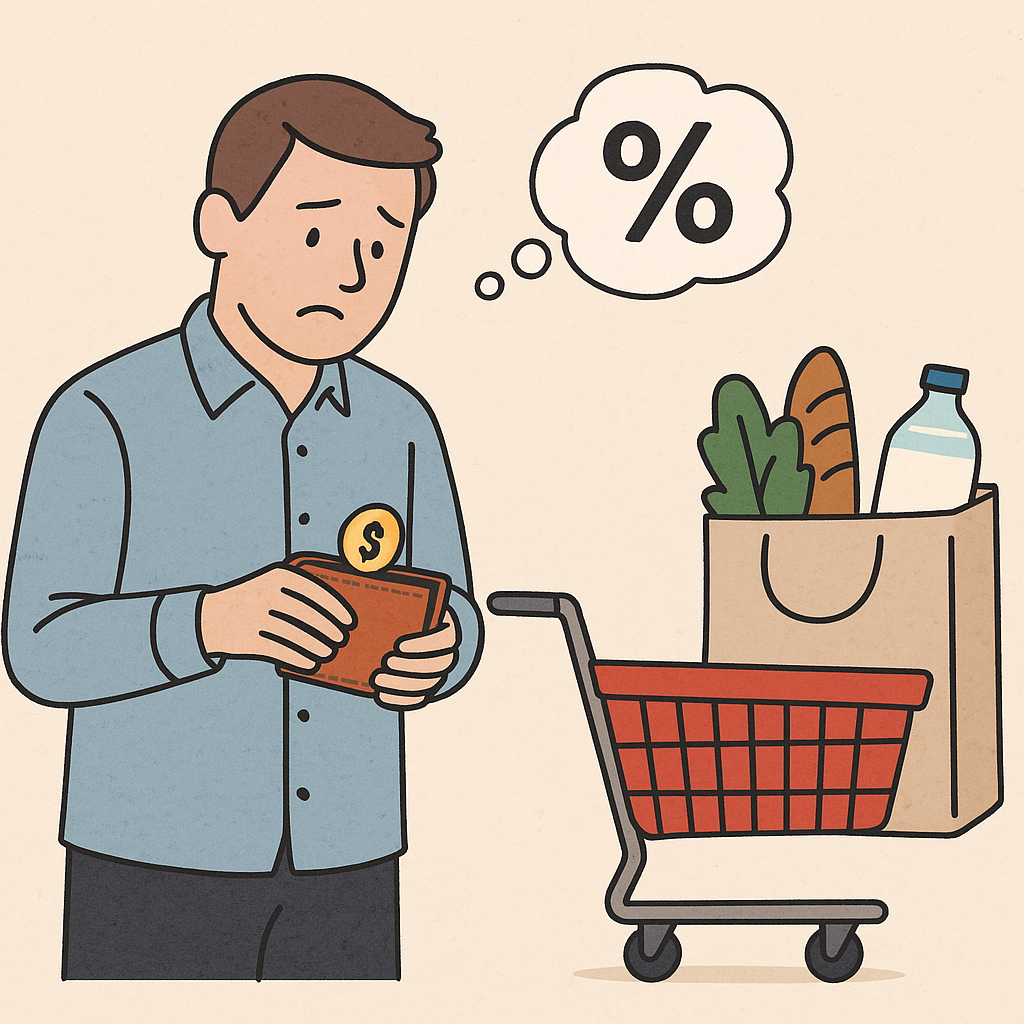
\includegraphics[width=\textwidth]{figuras/consumo2.png}
        \end{column}
        \begin{column}{0.5\textwidth}
            \centering
            \begin{itemize}
                \item Juros é o aluguel do dinheiro.
                \item Geralmente é usado para antecipar um consumo.
                \item Comprar com juros é pagar mais caro pelo mesmo produto.
                \item Pagar juros reduz seu poder de consumo.
            \end{itemize}
            % \textbf{\Large Juros é o aluguel do dinheiro}
        \end{column}
    \end{columns}
\end{frame}

% \begin{frame}[c]
%     \frametitle{}
%     \begin{columns}
%         \begin{column}{0.5\textwidth}
%             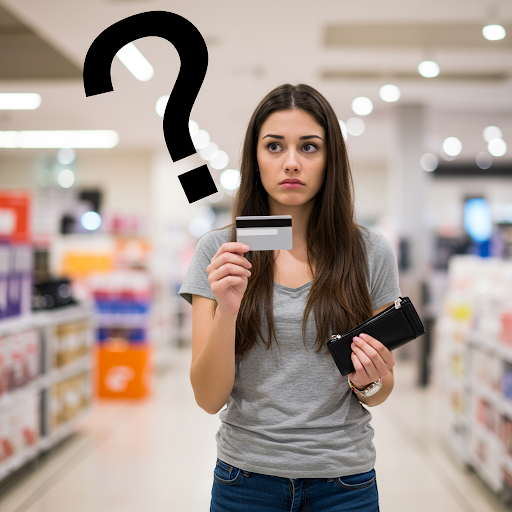
\includegraphics[width=\textwidth]{figuras/consumo3.png}
%         \end{column}
%         \begin{column}{0.5\textwidth}
%             \centering
%             \textbf{\Large Comprar com juros é pagar mais caro pelo mesmo produto.}
%         \end{column}
%     \end{columns}
% \end{frame}

% \begin{frame}[c]
%     \frametitle{}
%     \begin{columns}
%         \begin{column}{0.5\textwidth}
%             \centering
%             \textbf{\Large Quem paga juros reduz seu poder de consumo.}
%         \end{column}
%         \begin{column}{0.5\textwidth}
%             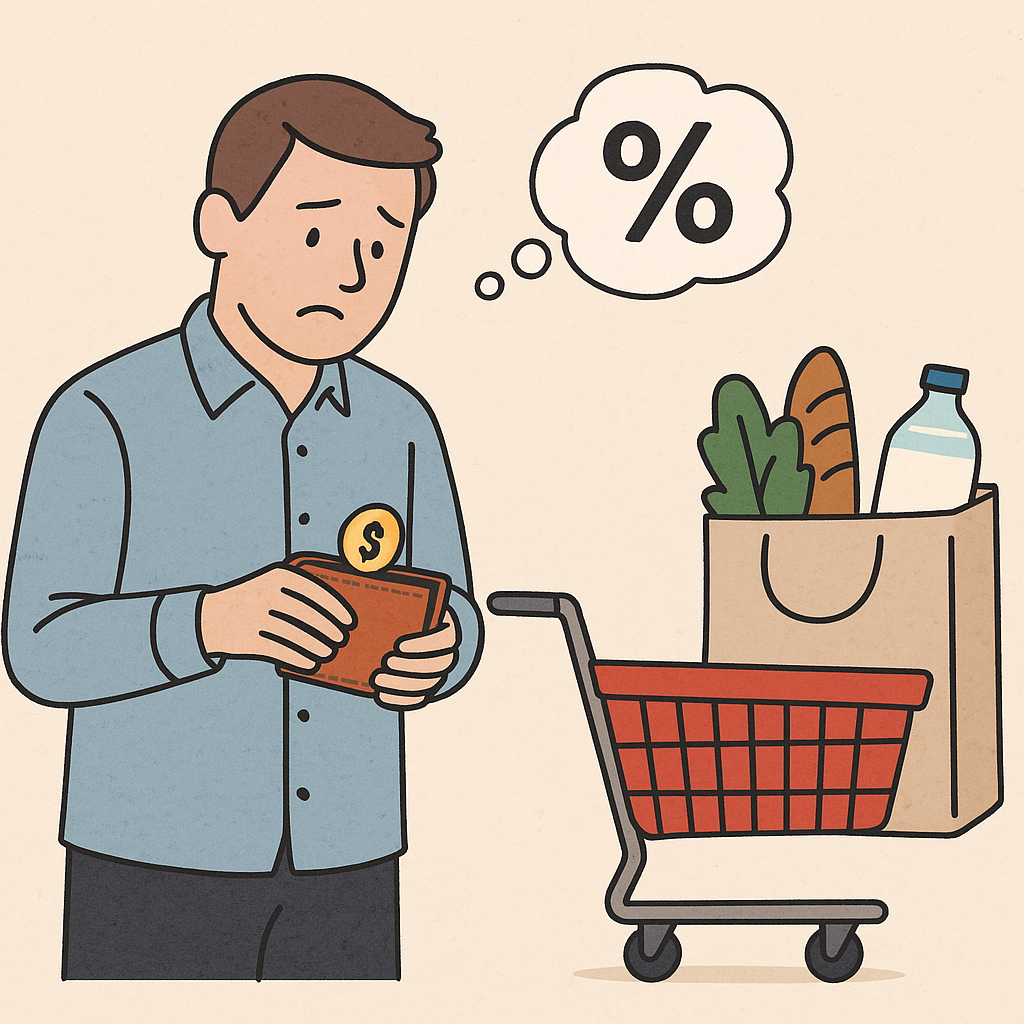
\includegraphics[width=\textwidth]{figuras/consumo2.png}
%         \end{column}
%     \end{columns}
% \end{frame}


% \begin{frame}[c]\frametitle{Podemos alugar nosso dinheiro para}
%     % \textbf{Minha Estratégia para quitar as dívidas}
%     \begin{itemize}
%         \item Bancos através de CDB, LCI, LCA, etc.
%         \item Governo através dos títulos do Tesouro Direto.
%         \item Empresas através de Debêntures.
%     \end{itemize}
% \end{frame}

\section{Quite suas dívidas primeiro}

\begin{frame}[c]\frametitle{Estratégia para quitar as dívidas e liberar o orçamento}
    \textbf{Plano de Ação}
    \begin{itemize}
        \item \textbf{Crie um Orçamento:} Ajuste seus gastos para que sejam sempre menores do que o seu ganho mensal.
        \item \textbf{Use Rendas Extras:} Direcione o 13$^\text{o}$ salário, adicional de férias e outros bônus exclusivamente para o pagamento das dívidas.
        \item \textbf{Busque Renda Extra:} Aumente sua receita mensal com trabalhos adicionais para acelerar a quitação.
        \item \textbf{Controle a Inflação do Estilo de Vida:} Não aumente seus gastos ao receber um aumento salarial. Use o valor extra para pagar as dívidas ou para investir.
    \end{itemize}
\end{frame}
% !TEX root = main.tex
\section{Ativos e Passivos: A Base para a Prosperidade Financeira.}

\begin{frame}[c]\frametitle{Ativos}
  \textbf{O que são Ativos?}
  \begin{itemize}
    \item São todos os bens e recursos que você possui e que geram renda ou se valorizam com o tempo.
  \end{itemize}

  \textbf{Exemplos de Ativos:}
  \begin{itemize}
    \item Investimentos (Ações, títulos, fundos, etc.)
    \item Imóveis
    \item Seu próprio negócio ou fonte de renda
    \item Tudo aquilo que te gera renda.
  \end{itemize}
\end{frame}

\begin{frame}[c]\frametitle{Passivos}
  \textbf{O que são Passivos?}
  \begin{itemize}
    \item São todas as obrigações financeiras que você tem a pagar, ou seja, tudo que tira dinheiro do seu bolso.
  \end{itemize}

  \textbf{Exemplos de Passivos:}
  \begin{itemize}
    \item Dívidas (empréstimos, financiamento de carro, cartão de crédito)
    \item Contas fixas (aluguel, condomínio, luz, internet)
    \item Impostos e juros
    \item Tudo aquilo que te gera despesa.
  \end{itemize}
\end{frame}


\begin{frame}[c]\frametitle{O Fluxo do Dinheiro}
  \begin{center}
    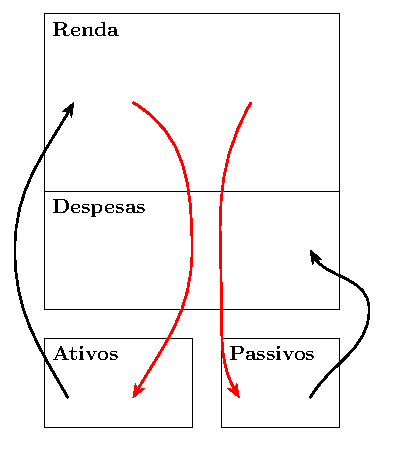
\includegraphics{../figuras/pai_rico}
  \end{center}
\end{frame}

\begin{frame}[c]\frametitle{O Impacto no Patrimônio}
  \begin{columns}
    \begin{column}{0.5\textwidth}
      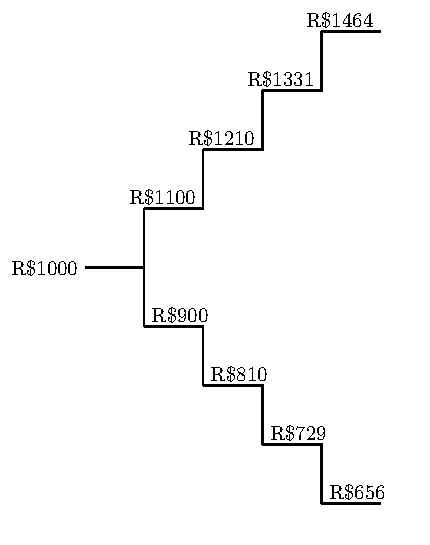
\includegraphics[width=\textwidth]{../figuras/dobra4.pdf}
    \end{column}
    \begin{column}{0.5\textwidth}
      \centering
      \textbf{\large Ao final de 4 anos um ativo rendendo de 10\% a.a. vale mais que o dobro de um passivo que desvaloriza na mesma taxa.}
      % \begin{itemize}
      %   \item Taxa de juros anual de 10\% a.a.
      %   \item $\frac{\text{R\$ 1464}}{\text{R\$656}} = 2,23$.
      %   \item Tentar gerar renda extra.
      %   \item Não aumentar os gastos devido a aumento salarial.
      % \end{itemize}
    \end{column}
  \end{columns}
\end{frame}

\begin{frame}[c]\frametitle{Exemplo Prático: A Compra um Carro}
  \textbf{Patrimônio Inicial:} R\$120.000,00

  \begin{itemize}
    \item \textbf{Cenário 1:} Gasta R\$100.000,00 na compra de um carro e investe o restante.
    \item \textbf{Cenário 2:} Gasta R\$60.000,00 na compra de um carro e investe o restante.
    \item \textbf{Cenário 3:} Não compra o carro e investe os R\$120.000,00.
  \end{itemize}

  \textbf{Premissas:}
  \begin{itemize}
    \item Desvalorização do carro: 10\% ao ano.
    \item Custo de Oportunidade: 12\% ao ano (quanto o dinheiro rende investido).
  \end{itemize}
\end{frame}

\begin{frame}[c]\frametitle{Analisando o Cenário 1}
  \textbf{Decisão: Comprar carro de R\$100 mil e investir R\$20 mil}
  \begin{itemize}
    \item \textbf{Patrimônio Inicial:} R\$ 120.000,00
    \item \textbf{Carro (depreciação de 10\% a.a.)}: R\$ 100.000,00
    \item \textbf{Saldo Investido (rendimento de 12\% a.a.)}: R\$ 20.000,00
  \end{itemize}
  \begin{center}
    \begin{tabular}{|c|c|c|c|}
      \hline
      \textbf{Ano} & \textbf{Valor do Carro} & \textbf{Valor Investido} & \textbf{Patrimônio Total} \\
      \hline
      \textbf{0}   & R\$ 100.000,00          & R\$ 20.000,00            & R\$ 120.000,00            \\
      \textbf{1}   & R\$ 90.000,00           & R\$ 22.400,00            & R\$ 112.400,00 (-6,33\%)  \\
      \textbf{2}   & R\$ 81.000,00           & R\$ 25.088,00            & R\$ 106.088,00 (-5,62\%)  \\
      \textbf{3}   & R\$ 72.900,00           & R\$ 28.098,56            & R\$ 100.998,56 (-4,80\%)  \\
      \textbf{4}   & R\$ 65.610,00           & R\$ 31.470,39            & R\$ 97.080,39  (-3,88\%)  \\
      \textbf{5}   & R\$ 59.049,00           & R\$ 35.246,83            & R\$ 94.295,83  (-2,87\%)  \\
      \hline
    \end{tabular}
  \end{center}
\end{frame}

\begin{frame}[c]\frametitle{Analisando o Cenário 2}
  \textbf{Decisão: Comprar carro de R\$60.000,00 e investir R\$60.000,00}
  \begin{itemize}
    \item \textbf{Patrimônio Inicial:} R\$ 120.000,00
    \item \textbf{Carro (depreciação de 10\% a.a.)}: R\$ 60.000,00
    \item \textbf{Saldo Investido (rendimento de 12\% a.a.)}: R\$ 60.000,00
  \end{itemize}
  \begin{center}
    \begin{tabular}{|c|c|c|c|}
      \hline
      \textbf{Ano} & \textbf{Valor do Carro} & \textbf{Valor Investido} & \textbf{Patrimônio Total} \\
      \hline
      \textbf{0}   & R\$ 60.000,00           & R\$ 60.000,00            & R\$ 120.000,00            \\
      \textbf{1}   & R\$ 54.000,00           & R\$ 67.200,00            & R\$ 121.200,00 (+1,00\%)  \\
      \textbf{2}   & R\$ 48.600,00           & R\$ 75.264,00            & R\$ 123.864,00 (+2,20\%)  \\
      \textbf{3}   & R\$ 43.740,00           & R\$ 84.295,68            & R\$ 128.035,68 (+3,37\%)  \\
      \textbf{4}   & R\$ 39.366,00           & R\$ 94.411,16            & R\$ 133.777,16 (+4,48\%)  \\
      \textbf{5}   & R\$ 35.429,40           & R\$ 105.740,50           & R\$ 141.169,90 (+5,53\%)  \\
      \hline
    \end{tabular}
  \end{center}
\end{frame}

\begin{frame}[c]\frametitle{Patrimônio Ano a Ano nos 3 cenários}
  \begin{center}
    \begin{tabular}{|l|c|c|c|}
      \hline
      \textbf{Ano} & \textbf{Cenário 1} & \textbf{Cenário 2} & \textbf{Cenário 3} \\
      \hline
      \textbf{0}   & R\$ 120.000,00     & R\$ 120.000,00     & R\$ 120.000,00     \\
      \textbf{1}   & R\$ 112.400,00     & R\$ 121.200,00     & R\$ 134.400,00     \\
      \textbf{2}   & R\$ 106.088,00     & R\$ 123.864,00     & R\$ 150.528,00     \\
      \textbf{3}   & R\$ 100.998,56     & R\$ 128.035,68     & R\$ 168.591,36     \\
      \textbf{4}   & R\$ 97.080,39      & R\$ 133.777,16     & R\$ 188.822,32     \\
      \textbf{5}   & R\$ 94.295,83      & R\$ 141.169,90     & R\$ 211.481,00     \\
      \hline
    \end{tabular}
  \end{center}
\end{frame}


\begin{frame}[c]\frametitle{Retorno Final após 5 anos}
  \begin{tabular}{|l|c|c|c|}
    \hline
    \textbf{Cenário}   & \textbf{Patrimônio Final} & \textbf{Retorno Total (R\$)} & \textbf{Retorno Total (\%)} \\
    \hline
    \textbf{Cenário 1} & R\$ 94.295,83             & -R\$ 25.704,17               & -21,42\%                    \\
    \textbf{Cenário 2} & R\$ 141.169,90            & +R\$ 21.169,90               & +17,64\%                    \\
    \textbf{Cenário 3} & R\$ 211.481,00            & +R\$ 91.481,00               & +76,23\%                    \\
    \hline
  \end{tabular}
\end{frame}
\section{Previdência Privada}

\begin{frame}[t]\frametitle{PGBL - Plano Gerador de Benefício Livre}
  \textbf{Características do PGBL:}
  \begin{itemize}
    \item Indicado para quem \textbf{declara o IR no modelo completo}.
    \item Permite \textbf{dedução de até 12\% da renda bruta anual} no IR.
    \item Tributação ocorre sobre \textbf{o valor total} (contribuições + rendimentos) no resgate.
    \item Pode ser vantajoso para quem tem renda mais alta e deseja reduzir o imposto a pagar no presente.
  \end{itemize}
\end{frame}

\begin{frame}[t]\frametitle{VGBL - Vida Gerador de Benefício Livre}
  \textbf{Características do VGBL:}
  \begin{itemize}
    \item Indicado para quem \textbf{declara o IR no modelo simplificado} ou é \textbf{isento}.
    \item Não permite dedução das contribuições no IR.
    \item Tributação ocorre apenas sobre \textbf{os rendimentos} no resgate.
    \item Mais vantajoso para quem não pode ou não quer aproveitar o benefício fiscal do PGBL.
  \end{itemize}
\end{frame}

\begin{frame}[t]\frametitle{Tributação Regressiva na Previdência Privada}

  \vspace{0.5cm}
  \textbf{Tabela de Alíquotas:}

  \begin{table}[]
    \centering
    \begin{tabular}{|c|c|}
      \hline
      \textbf{Tempo de Investimento} & \textbf{Alíquota de IR} \\ \hline
      Até 2 anos                     & 35\%                    \\ \hline
      De 2 a 4 anos                  & 30\%                    \\ \hline
      De 4 a 6 anos                  & 25\%                    \\ \hline
      De 6 a 8 anos                  & 20\%                    \\ \hline
      De 8 a 10 anos                 & 15\%                    \\ \hline
      Acima de 10 anos               & 10\%                    \\ \hline
    \end{tabular}
  \end{table}
\end{frame}

\begin{frame}[t]\frametitle{Exemplo: PGBL e Benefício Fiscal}
  \textbf{Situação Inicial:}
  \begin{itemize}
    \item Base de cálculo do IR: \textbf{R\$ 100.000}
    \item Alíquota marginal de IR: \textbf{27,5\%}
  \end{itemize}

  \vspace{0.3cm}
  \textbf{Após o Aporte no PGBL:}
  \begin{itemize}
    \item Aporte: \textbf{R\$ 10.000}
    \item Nova base de cálculo: \textbf{R\$ 90.000}
    \item \textbf{Economia de imposto: R\$ 2.750}
  \end{itemize}
\end{frame}




% --------------------------------------------------------------------------------------------------
\begin{frame}[c]\frametitle{}
  \begin{center}
    \LARGE \textcolor{UFGblue}{\textbf{Obrigado por sua atenção!}}
  \end{center}
\end{frame}
% --------------------------------------------------------------------------------------------------
\end{document}

